\documentclass [12pt,letterpaper]{article}
\usepackage[margin=1.3in]{geometry}
\usepackage{graphicx, lscape, url}
\usepackage{wrapfig}

\setlength\parindent{0pt}

\begin{document}
 
% Titlepage
\thispagestyle{empty}
\begin{center}
    \centering
% University logo
    
\includegraphics[width=0.3\linewidth]{images/nottingham-logo.png}
    \vspace{0.1cm}
    {\Large \\University of Nottingham\par}
    {\Large Department of Computer Science\par}
    \vspace{3cm}
% Project title
    {\Large COMP3003 - Interim Report\par}
    \vspace{0.5cm}
    {\Large A Cross-platform Networking Configuration \& Auditing Mobile Application\par}
    \vspace{2.5cm}
% Author Name
    {\Large Jozef W. Sieniawski\par}
    {\small Computer Science BSc. \par}
    {\small 20296126 $|$ psyjs25@nottingham.ac.uk\par}
    \vspace{1cm}
% Supervisor
    {\normalsize Supervisor: Proff. Chris Greenhalgh\par}
    \vspace{3cm}
% Date
    {\Large September 2022}
\end{center}

\pagebreak
\begin{abstract}
For Small/Medium, and even some large, companies that own and maintain their own server spaces, a unique set of challenges are to be faced. Although these devices are typically business critical, they are typically squeezed into encumbered spaces, with lackluster lighting and limited access. Further, and critically, this makes the maintaining and documenting of these devices inherently more difficuly. Current alternative solutions fail to focus on insitu use, and are typically bloated with features for large data centers. This project investigates the needs and requirements that can solves these challenges, with a focus on Human-Computer Interaction. From these designs, this project then implements a cross-platform mobile application that satisfies these needs.
\end{abstract}
% Table of contents
\pagebreak
\tableofcontents
\pagebreak 

% Add spacing between paragraphs
\setlength{\parskip}{2ex}

% Introduction
\section{Introduction}
\label{sec:introduction}
With the work for the Research Support Team in the School of Computer Science at Nottingham, one of the primary responsibilities revolves around server spaces. This involves the installation and configuration of new servers, as well as the maintenance of existing hardware. When we were faced with the task of migrating servers to a new location, the problem of understanding the configuration of the existing servers arose. There lacked a consistent documentation format that could be used to replicate the configuration of a server in a new location.

With a larger project in mind, where understanding the configuration of many servers was essential, the idea of this project was born; To create a tool that will allow for cable configuration of server hardware to be easily digitised, visualised, queried and updated.

Whilst alternatives exist, they are typically a segment of a far larger suite of tools, which are usually not necessary for small/medium sized server spaces. Naturally, cable configurations can be difficult to understand and work with even in these smaller spaces. This also brought forward the second aspect of the project, to also be an investigation into the user experience and interface design of the tool. To ensure that the tool is easy to use and can be understood by a wide range of users.

Further, the project will be open source, and will be available for use by the wider community of server administrators. This will allow for the human Computer interaction findings that have been implemented to be used in similar applications. Additionally, the tool will be utilising and integrating with Netbox, an open-source tool for managing network infrastructure. This will act as the backing database for the tool and will allow for the tool to be used in a wider context of server management.

The Research Support Team will act as a prime example of the target audience. The project aims to discover the needs of a wider range of small and medium sized enterprises (SME) who run and maintain their own server spaces. As mentioned previously, there are not many similar alternatives to the project as these SME's usually pose a unique server environment. These spaces can be cramped, poorly lit and hard to navigate. Seen below is a picture of the server space in the School of Computer Science at Nottingham (fig. 1), which is an example of the type of environment that the project will be designed for.

\begin{figure}[ht]
    \centering
    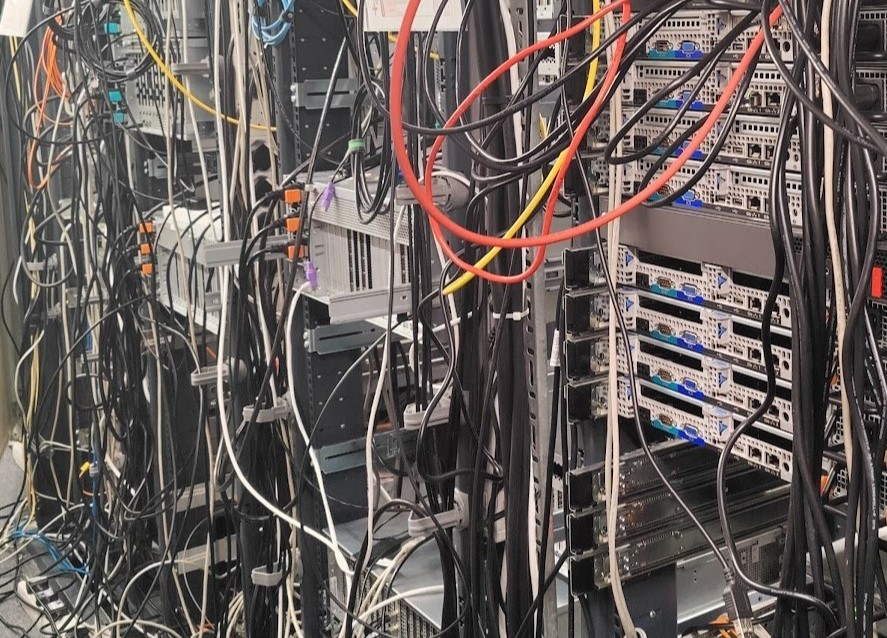
\includegraphics[width=0.4\linewidth]{images/server_racks.jpg}
    \caption{Server Rack within the school of Computer Science}
\end{figure}

This is another reason that typical solutions cannot usually apply to these spaces, as they are often designed for large data centres, where laptops can be used easily to use software in situ. A tool that can be used on a mobile device in these less-than-ideal conditions is something worthy of investigation. As mentioned, a perfect example of this is the server space in the School of Computer Science seen a (fig. 1). Before upgrades, the space was poorly lit and is, still relatively cramped. It’s not particularly feasible to use a laptop in this space comfortably, which most solutions rely on due to cluttered UI. The current layout of servers and hardware makes tracking cables completely impracticable and a mobile application would be a perfect solution to this problem. 


\begin{figure}[ht]
    \centering
    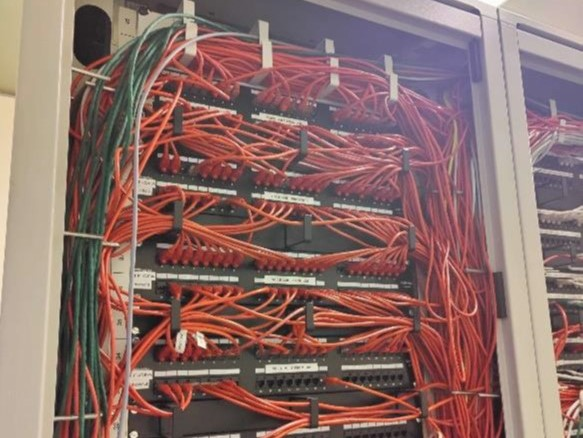
\includegraphics[width=0.4\linewidth]{images/server_racks_clean.jpg}
    \caption{More ideal and realistic server space}
\end{figure}

Comparatively, the server space dedicated to networking has been managed to a more ideal state (fig. 2). Whilst not perfect, comparing to that of data centers, it is far more manageable. This is the aim of the project, to create a tool that can be used in these less-than-ideal conditions to allow for scenarios like the one in fig. 1 to be managed more easily.


\subsection{Background}
\label{sec:background}
\subsection{Aims}
\label{sec:aims}
\subsection{Objectives}
\label{sec:objectives}
\subsection{Scope}
\label{sec:scope}
\section{Related Work}
\subsection{App Review}
\section{Description of the Work}

\section{Methodology}
\section{Design and Implementation}
All practicle stuff done
\subsection{Technical Work Done To Date}

\section{Progress}
\subsection{Projection Management}
\subsection{Contributions and Reflections}

% Bibliography
\pagebreak
\bibliographystyle{ieeetr}
\bibliography{citation} 
% Document End
\end{document}